\documentclass[a4paper,doc,natbib,floatsintext]{apa6}
\usepackage[english]{babel}
\usepackage[utf8x]{inputenc}
\usepackage{amsmath}
\usepackage{graphicx}
\usepackage{epstopdf}
\usepackage{url}
\usepackage{mathtools}
\usepackage{csquotes}
\usepackage[hidelinks]{hyperref}
\usepackage{subfigure}
\usepackage{booktabs}
\usepackage[section]{placeins}
\usepackage[sc]{mathpazo}
\usepackage{caption}
\captionsetup[table]{skip=8pt}
\usepackage{authblk}


% ---------- watermark -----------
\usepackage[firstpage]{draftwatermark}
\SetWatermarkAngle{0}
\SetWatermarkFontSize{0.25cm}
\SetWatermarkVerCenter{1.15cm}
\SetWatermarkLightness{0.5}
\SetWatermarkHorCenter{14cm}
\SetWatermarkText{\shortstack[l]{
De Deyne, S., Navarro, D. J., Perfors, A., Brysbaert, M. and Storms, G. (2019). \\
The Small World of Words: English word association norms for over 12,000 cue \\
words. Behavior Research Methods, 51, 987-1006 \\
https://doi.org/10.3758/s13428-018-1115-7
}}
\SetWatermarkScale{1}
% -------------------------------

\urlstyle{same}
\newcommand{\stim}[1]{\textsl{#1}}

\title{The ``Small World of Words'' English word association norms for over 12,000 cue words.}


\shorttitle{English Word Associations}

\author[1]{Simon De Deyne}
\author[2]{Danielle J. Navarro}
\author[1]{Amy Perfors}
\author[3]{Marc Brysbaert}
\author[4]{Gert Storms}
\affiliation{\hspace{1cm}}
\affil[1]{\small University of Melbourne, School of Psychological Sciences, 3010 VIC, Australia}
\affil[2]{\small University of New South Wales, School of Psychology, 2052 NSW, Australia}
\affil[3]{\small Ghent University, Department of Psychology, 9000 Ghent, Belgium}
\affil[4]{\small KU Leuven, Department of Psychology, 3000 Leuven, Belgium}


\keywords{Word associations, mental lexicon, networks, similarity, spreading activation}

\authornote{
This research was supported by ARC grant DE140101749 awarded to Simon De Deyne.
Our gratitude goes to all volunteers without whom none of this would have been possible. Special thanks to researchers who supported this project, in particular ConCat, Emmanuel Keuleers and Pawel Mandera for extra exposure, Max Louwerse for valuable discussion, James Deese and Douglas Nelson for continuous inspiration, and Jim Neely and Erin Buchanan for their helpful reviews. All comments can be sent to the first author.}

\abstract{
Word associations have been used widely in psychology, but the validity of their application strongly depends on the number of cues included in the study and the extent to which they probe all associations known by an individual. In this work, we address both issues by introducing a new English word association dataset. We describe the collection of word associations for over 12,000 cue words, currently the largest such English-language resource in the world. Our procedure allowed subjects to provide multiple responses for each cue, which permits us to measure weak associations. We evaluate the utility of the dataset in several different contexts, including lexical decision and semantic categorization. We also show that measures based on a mechanism of spreading activation derived from this new resource are highly predictive of direct judgments of similarity. Finally, a comparison with existing English word association sets further highlights systematic improvements provided through these new norms.}

\begin{document}
\maketitle

\section{Introduction}
The ``word association game'' is deceptively simple: you are presented with a word (the cue), and you have to respond with the first word that comes to mind. Playing the game feels effortless, automatic and often entertaining. Generating a word associate is easy and indeed, responding with a word that is \textit{not} the first thing that comes to mind turns out to be quite difficult \citep{Playfoot2016}. The simplicity of the task makes it an attractive methodological tool, and a remarkably powerful one: word associations reveal mental representations that cannot be reduced to lexical usage patterns, as the associations are free from the basic demands of communication in natural language \citep{Szalay1978,Prior2008,Mollin2009}.
As a technique, it is closely related to other subjective fluency tasks like the semantic feature elicitation task \citep{McRae2005,Vinson2008} and various category fluency tasks \cite[e.g.,][]{Battig1969} in which participants list as many exemplars for a category such as animals within a 1-min period.
Relative to other tasks, however, the word association technique provides us with a more general and unbiased approach to measure meaning \citep{Deese1965}. This means that a variety of stimuli can be used as cues, regardless of their part-of-speech or how abstract or concrete they are. Taken together, these properties make word associations an ideal tool to study internal representations and processes involved in word meaning and language in general.

In this paper we present a new and comprehensive set of word association norms from the \textit{English Small World of Words} project (SWOW-EN)\footnote{See \url{https://smallworldofwords.org}}. The data were collected between 2011 and 2018 and consist of +12,000 cue words and judgments from over 90,000 participants. This makes it comparable in size to a similar project in Dutch \citep{DeDeyne2013b} and substantially larger than any existing English-language resource.

The collection and usage of word association norms have a long history. One of the most widely used resources comes from the \textit{University of South Florida norms} \citep[USF norms,][]{Nelson2004}. Although it first appeared in 2004, it has been cited over 1900 times and is still the most commonly used resource in English. The collection of these norms started more than 40 years ago and involved over 6,000 participants. They contain single-word association responses from an average of 149 participants per cue for a set of 5,019 cue words\footnote{Most of this work was done by hand, and a vivid account of this ordeal is available at \url{http://w3.usf.edu/FreeAssociation/Intro.html}}. Another commonly used resource is the \textit{Edinburgh Associative Thesaurus} \cite[EAT;][]{Kiss1973},  a dataset collected between 1968 and 1971. It consists of 100 responses per cue for a total of 8,400 cues. More recently, British English word associations have also been collected as part of the \textit{Birkbeck norms} which contain 40 to 50 responses for over 2,600 cues \citep{Moss1996}. Looking beyond English, there are word association datasets with 1,000+ cues available in other languages including Korean \cite[3,900 cues;][]{Jung2010} and Japanese \cite[2,100 cues;][]{Joyce2005}.
The largest collection is available for the Dutch language (SWOW-NL) for which the most recently released dataset consists of over 12,000 cues \citep{DeDeyne2013b} and the latest iteration contains data for over 16,000 cues. This last dataset uses the same procedure as the one described here.

The remainder of the paper consists of two parts. In the first part we describe the new dataset and its properties. In the second part we evaluate the validity of these data, focusing on measures of lexical centrality and semantic similarity. Doing so allows us to demonstrate two ways in which we believe these data have broad applicability in the field, capitalizing on its unique scale (in terms of number of cues) and depth (in terms of number of responses).

\section{Data Collection}
The data described in this paper are part of an ongoing study to map the human lexicon in major languages of the world. Across these different languages, we have tried to keep the procedure as closely matched as possible. The original data collection project began in 2003 in Dutch \citep{DeDeyne2008a,DeDeyne2013b}, and since that time some minor changes have been implemented. First, although the earliest data collection relied on pen and paper tasks, the majority of the data collection for it (and all of the data collection for this project) has relied on a web-based task.
Over the time frame of the project we also implemented minor cosmetic changes to the website to enhance readability and to accommodate changes in web technology. Most notably, recent versions of the website have accommodated a wider variety of devices, reflecting changes in Internet usage in which more people rely on mobile devices. In response to interest from other researchers, we also decided to add a question about participant education levels at a point where the study was already underway. Minor alterations notwithstanding, the core word association task has remained unchanged throughout the project --- one in which the overriding consideration has been to keep the task short, simple, and inclusive.

\subsection{Method}
\subsubsection{Participants}
Participants were recruited online, using a crowd-sourced approach that relied on social media, e-mail and university websites. No restrictions were placed on participating apart from the requirement that participants be a fluent English speaker. People interested in participating despite a lack of English fluency were referred to other languages in the Small World of Words project as appropriate (currently 14 languages are included).

While there were no age restrictions, only data for participants aged 16 years and above were used, as we were mainly interested in the representation of a mature lexicon. The participants consisted of 88,722 volunteers, of whom 54,712 (62\%) identified as female, 33,710 (38\%) identified as male, and 300 (<1\%) responded using the unspecified gender category. The average age was 36 years ($SD$ = 16).
Besides gender and age, we also collected information about the native language of the participants. This was done in two steps. First, we asked the participants to indicate whether they were a native speaker of English. Depending on their answer, they were able to choose from a list of English-speaking regions, or from a list with most non-English languages spoken in the world. Most people (81\%) were native American English speakers (50\%), with British (13\%) Canadian (11\%) and Australian (5\%) speakers as next three largest groups represented in the data. In 2013 we also began collecting information about level of education, so these data are available for 40\% of the participants. Most of our participants had at least a college or university bachelor (81\%) or master degree (37\%). This suggests a fairly homogeneous sample in terms of education, with some degree of selection bias evident.


\subsubsection{Materials}

Stimulus materials (cue words) were constructed using a snowball sampling method, allowing us to include both frequent and less-frequent cues at the same time. The procedure also allowed us the flexibility to add cue words that were part of other published studies, which we did over the course of seven different iterations over the years.
The final set consisted of 12,292 cues included all 1,661 primes and targets from the Semantic Priming Project of \cite{HutchisonBalota2013}, all 5,019 cues from the University of South Florida norms \citep{Nelson2004} and most of the cues that were part of previously published English word modality norms \citep{LynottConnnell2013} and semantic feature production norms \citep{McRae2005}.

\subsubsection{Procedure}
The study was approved by the KU Leuven Ethics Committee (ref. G-2014 07 017), and the procedure was identical to the Dutch language data (SWOW-NL) reported by \citet{DeDeyne2008a} and \citet{DeDeyne2013b}. Participants were instructed that a word would appear on the screen and they were asked to respond with the first three words that came to mind. If they could not think of any further responses, they could indicate this by pressing the ``No More Response'' button. If a word was unknown, they were asked to select the ``Unknown Word'' button. They were also instructed to respond only to the word displayed on top of the screen (not to their previous responses) and to avoid typing full sentences as responses. Each participant was presented with a list of 14 to 18 stimuli. The stimuli presented were selected randomly from those cues with the fewest responses in the current iteration. Each stimulus appearing on the screen was followed with a form consisting of three text fields, one for the first (R1), second (R2), and third (R3) response. Once a field was completed by pressing enter or clicking a button, that entry could no longer be changed. The response remained on the screen but the color of the response was changed from black to gray.

\subsection{Data preprocessing}
The data were normalized in a number of steps. We first removed tags, quotes, final punctuation, and double spaces. In some cases, participants indicated unknown words or missing responses literally rather than pressing the button. For example, people sometimes typed \stim{unknown word}, \stim{no response}, or \stim{?}\  rather than pressing the labeled buttons. These responses were recoded as ``Unknown word'' and missing (``No more responses'') responses.
Only unique responses were included, with duplicate responses to a specific cue by the same participant recoded as missing responses. This affected 3,222 responses. Next, a small number of cues were recoded, which will be discussed in the coming paragraphs.
In what follows, we will focus on American English, as most of the participants spoke this variant. A basic flowchart outlining the various steps of filtering the data is presented in Figure~\ref{figure:flowchart}.

\subsubsection{Exclusions}
We excluded participants from the dataset if they did not meet our a priori criteria.
First, we excluded participants that used short sentences. This was determined by counting the number of verbose responses ($n$-gram with $n > 1$) and removing those participants where more than 30\% of the responses consisted of these $n$-grams (2,088 or 2.4\% of participants).\footnote{Participants might match multiple removal criteria simultaneously. The numbers reported here do not consider overlapping matches, but report only the number of participant matching each criterion separately.}
We excluded participants for whom fewer than 80\% of the responses were unique (i.e., they gave the same response to many different cue words, 754 or 0.8\% of participants).
We also removed participants with fewer than 60\% of their responses appearing on an English word list. The word list was compiled by combining word forms occurring at least twice in the English SUBTLEX \citep{BrysbaertNew2009} combined with the spelling list of American English extracted from the VarCon list \citep{Atkinson:2018} and a list of spelling corrections used in this study (see infra). This removed 1,201  or 1.4\% of the participants.
Finally, participants who indicated that they did not know more than 60\% of their words were also excluded. This removed 1,815 (2.0\%) of the participants.
Although the goal of data collection was to recruit 100 participants for every cue word, the logistics of large scale data collection mean that there were some cases in which this number was exceeded. For consistency, the current release of the SWOW-EN dataset includes only 100 participants per cue. In those cases where more than 100 responses were available for a cue, we preferentially included data from fluent speakers from major countries in the English-speaking world (Australia, Canada, Jamaica, New Zealand, Puerto Rico, United Kingdom, United States of America, Republic of Ireland, and South Africa). As a result, a total of 177,120 responses are not further considered in this report and the final dataset then consisted of 83,864 participants and 3,684,600 responses.


\begin{figure}[t]
\centering
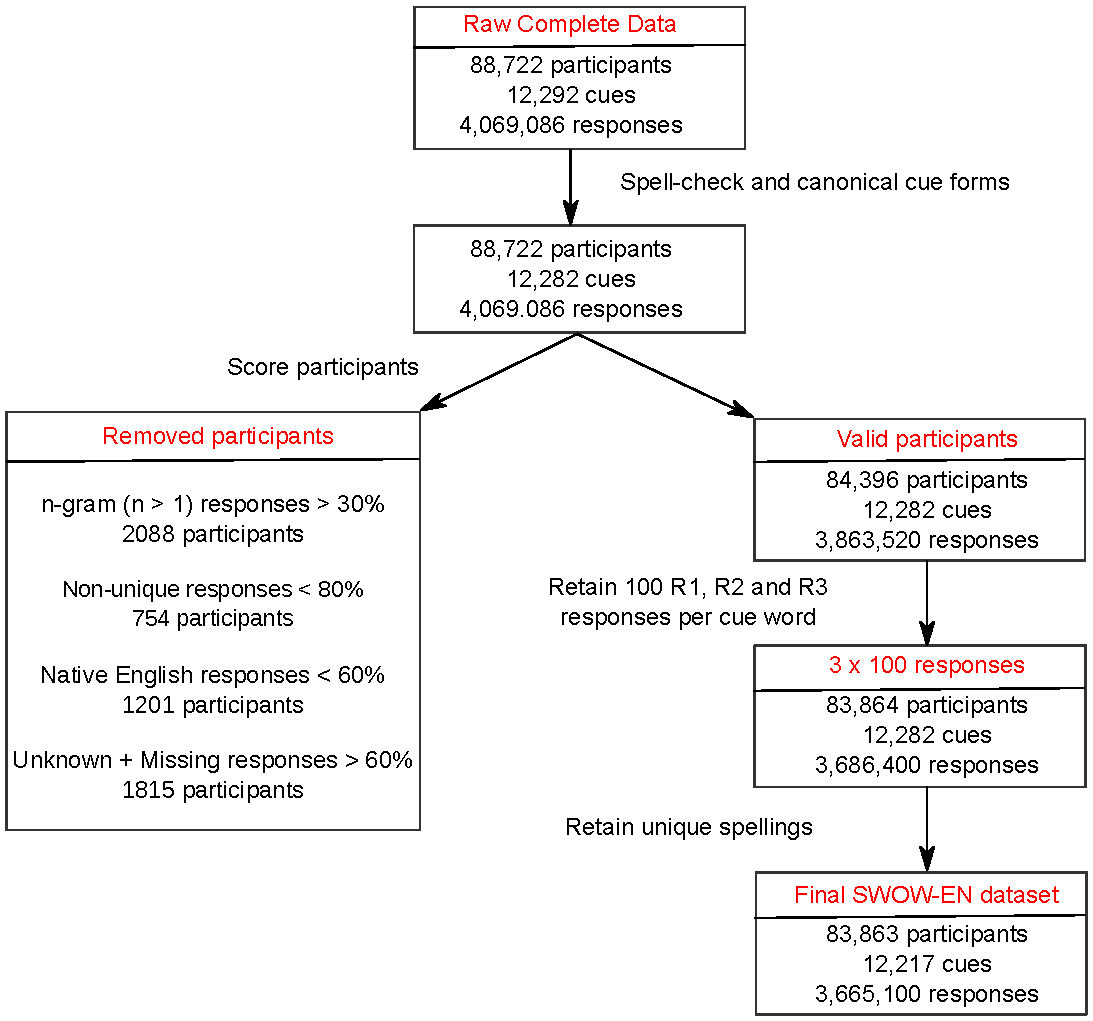
\includegraphics[width=0.7\textwidth]{figures/flowChartPreprocessing.pdf}
\caption{\small{A simplified flowchart providing a schematic overview of how the preprocessing steps affected the number of participants, cues and responses.}}
\vspace{0.1cm}
\label{figure:flowchart}
\end{figure}


\subsubsection{Canonical forms}
Following pre-processing and participant screening, all responses were recoded in a more canonical form. For nouns we removed both indefinitive and definitive particles (\stim{a} and \stim{the}, respectively). For verbs we removed the infinitival particle \stim{to}. Some responses suggest explicit word completions because participants preceded their response with a hyphen (-) or ellipsis (...).
To be able to interpret these responses, we added the cue word as part of the response (e.g., if the cue word was \stim{pot} and the response was \stim{-ato} it was recoded as \stim{potato}). Similarly, we corrected responses (and occasionally cues) that unambiguously referred to proper nouns, but were spelled with lower case (e.g., \stim{lego} becomes \stim{Lego}). More generally, to the best of our ability we manually spell-checked all responses occurring at least two times and added proper capitalization in cases that were mostly unambiguous.

\subsubsection{Multiple spellings}
Our goal is to provide a resource which can be used in a uniform way across a broad range of studies. One of the trade-offs we face is how to deal with regional variations in spelling found in UK, Australian, Canadian and other forms of English besides American English. In the remainder of the article we focus on American English (spell-checked) responses, leaving room to re-analyze and further collect data in future work and making the raw uncorrected data available as well, which might be of interest when studying spelling difficulties.

In practice this led to the following changes. There are a number of words that appeared as cues in multiple forms corresponding to regional spelling variations (e.g., \stim{odor} and \stim{odour}), and in such cases we included only the American English variant. Accordingly, our analyses did not consider \stim{aeroplane}, \stim{arse}, \stim{ax}, \stim{bandana}, \stim{bannister}, \stim{behaviour}, \stim{bellybutton}, \stim{centre}, \stim{cheque}, \stim{chequered}, \stim{chilli}, \stim{colour}, \stim{colours}, \stim{corn-beef}, \stim{cosy}, \stim{doughnut}, \stim{extravert}, \stim{favour}, \stim{fibre}, \stim{hanky}, \stim{harbour}, \stim{highschool}, \stim{hippy}, \stim{honour}, \stim{hotdog}, \stim{humour}, \stim{judgment}, \stim{labour}, \stim{light bulb}, \stim{lollypop}, \stim{neighbour}, \stim{neighbourhood}, \stim{odour}, \stim{oldfashioned}, \stim{organisation}, \stim{organise}, \stim{paperclip}, \stim{parfum}, \stim{phoney}, \stim{plough}, \stim{practise}, \stim{practise}, \stim{programme}, \stim{pyjamas}, \stim{racquet}, \stim{realise}, \stim{recieve}, \stim{saviour}, \stim{seperate}, \stim{smokey},\stim{theatre}, \stim{tresspass}, \stim{tyre}, \stim{verandah}, \stim{whisky}, \stim{WIFI}, and \stim{yoghurt}. These cue words and their responses were removed and only the American cue variant was retained.
Some cues also occurred with or without spaces or dashes (e.g., \stim{bubble gum} and \stim{bubblegum}). We replaced \stim{black out}, \stim{break up}, \stim{breast feeding}, \stim{bubble gum}, \stim{cell phone}, \stim{coca-cola}, \stim{good looking},\stim{goodlooking},\stim{good looking},\stim{hard working},\stim{hard-working}, \stim{lawn mower}, \stim{seat belt} and \stim{tinfoil} with \stim{blackout}, \stim{breakup}, \stim{breastfeeding}, \stim{bubblegum}, \stim{cellphone}, \stim{Coca Cola}, \stim{good-looking},\stim{hardworking},\stim{lawnmower}, \stim{seatbelt} and \stim{tin foil}.
For consistency, we also replaced two cues that only occurred with British spelling, \stim{aeon} and \stim{industrialise}, with their American counterparts, \stim{eon} and \stim{industrialize}. Finally, we changed  \stim{bluejay}, \stim{bunk bed}, \stim{dingdong}, \stim{dwarves}, \stim{Great Brittain}, \stim{lightyear}, \stim{manmade}, \stim{miniscule}, and \stim{pass over} to \stim{blue jay}, \stim{bunkbed}, \stim{ding dong}, \stim{dwarfs}, \stim{Great Britain}, \stim{light year}, \stim{man-made}, \stim{minuscule} and \stim{passover}. Along the same lines, for the purposes of analysis, we Americanized all non-American spellings in the response data. The resulting dataset reduced the original 12,282 cues to 12,218 cue words.


\subsection{Distributional properties of cues and responses}
Our initial look at the data examines how responses are distributed across cues: how often do people produce idiosyncratic ``hapax legomena'' responses? How does the number of types (unique words) increase as a function of the number of tokens (unique responses) in the data? How often are people unable to produce a response?

\subsubsection{Types and tokens} Aggregating across all three responses, there were 133,762 distinct word forms (types) produced in the dataset, of which only 76,602 appeared only once. If we restrict ourselves to the first response, there are 64,631 types, of which 33,410 words occurred only once. Those responses that occur only once are referred to as \textit{hapax legomena} responses. While these are sometimes removed \citep{Nelson2004}, our approach is to retain these, in line with the Dutch SWOW data from \citet{DeDeyne2013b}. This approach reflects the view that these are not unreliable responses but simply reflect the long tail of the frequency spectrum. Of the first responses (R1), 2.8\% of the total number of response tokens and 51.7\% of response types were hapax legomena; when we consider all three responses (R123), the percentages are similar (2.3\% of tokens and 57.3\% of types). The ten most frequent types and tokens for R1 and R123 are shown in Table~\ref{Table:ResponseExamples}. Regardless of how frequency was calculated, most words in the top ten were the same.

\begin{figure}[t]
\centering
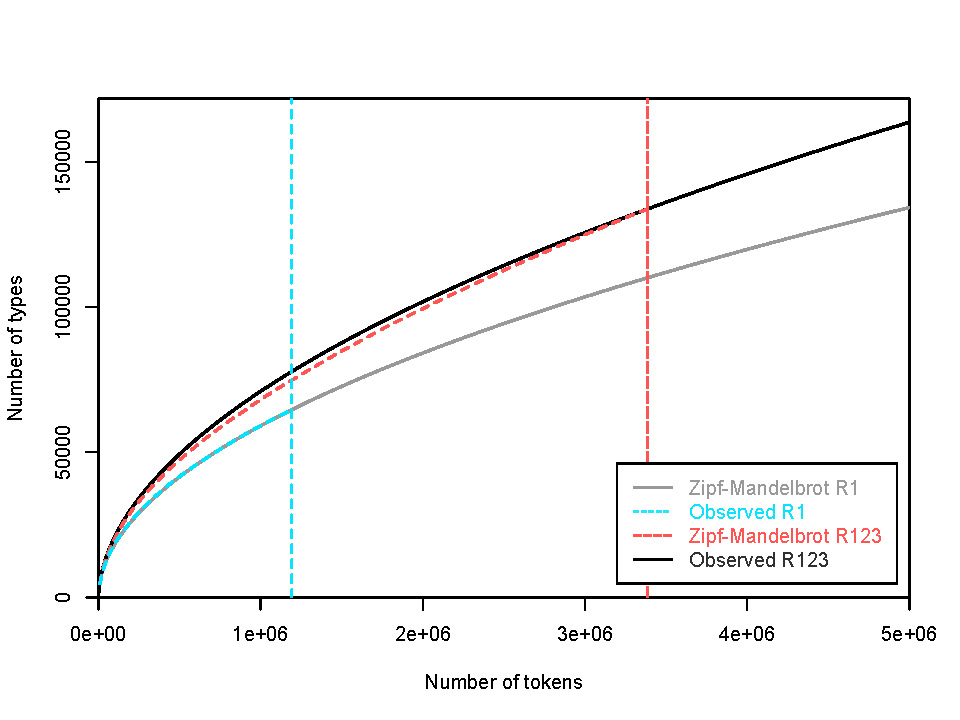
\includegraphics[width=0.7\textwidth]{figures/VocabularyGrowth.pdf}
\caption{\small{Vocabulary growth curve comparing the empirical or observed growth with the estimates from a finite Zipfian Mandelbrot (fZM) model \citep{evertbaroni}. The curves show how the number of different types (y-axis) increase as a function of the number of response tokens (x-axis).
The vertical lines indicate the total number of observed tokens for R1 and R123.
The productivity of human language is evident in the fact that regardless of the sample size, new word types are continuously produced. This effect is greatest when including second and third responses (R123) rather than only first responses (R1).}}
\label{figure:VocabularyGrowth}
\end{figure}


In natural language, the number of word types is boundless, as new words are coined all the time. This is captured by Herdan's law which describes an empirical exponential relation between the number of distinct words and the size of the text (the so called type-token ratio). According to Herdan's law we might expect that the number of distinct responses in the word association task also increases as we collect more data, although the number of new responses will gradually drop as the dataset gets larger \citep{Herdan1964}.

To provide a sense of how the number of distinct cue-response pairs (types) increases as a function of the total number of responses tokens, we estimated vocabulary growth curves for the first response data (R1) and the complete dataset (R123). The results are shown in Figure~\ref{figure:VocabularyGrowth}, which plots the number of types observed as a function of the number of tokens examined for the empirical data (solid lines). Because there are three times as many responses in R123 as in R1, we fit a finite Zipfian Mandelbrot model to both datasets using the {\it zipfR} package \citep{evertbaroni}. Perhaps unsurprisingly, the model fit curves (dashed lines in Figure~\ref{figure:VocabularyGrowth} show that the number of new types steadily increases as a function of the number of tokens collected. The continued growth in the curve highlights the productive nature of human language: there appears to be no adequate sample size to capture all words in a language. More interesting perhaps is the fact that the rate with which new types are added is \textit{higher} for the R123 data than for the R1 data, reflecting the fact that the second and third responses do not merely constitute \textit{more} data, they also elicit different responses from R1. As we will see in later sections, this increased response heterogeneity results in denser networks that produce better estimates of various kinds of language-related behavior.


\begin{table}[t]
\centering
\caption{The ten most frequent response words, calculated using the first response (R1) data only or aggregating over all three responses (R123). In the ``types'' column, frequency is defined as the total number of cue words for which the response was produced at least once. That is, the types-based measure ignores the strength of the association and merely looks at the number of cues to which the response is associated, whereas the tokens-based measure is sensitive to the number and strength of the associations. For the ``tokens'' columns, frequency is measured as the total number of times that the response word was produced.}
\label{Table:ResponseExamples}
\begin{tabular}{@{}cccccc@{}}
\toprule
\multicolumn{2}{c}{\textbf{Types}}      &        & \multicolumn{2}{c}{\textbf{Tokens}}               &                      \\
\midrule
\multicolumn{1}{c}{R1} & \multicolumn{1}{c}{R123} & \multicolumn{1}{c}{} & \multicolumn{1}{c}{R1} & \multicolumn{1}{c}{R123} \\
\cmidrule(r){1-2} \cmidrule(lr){4-5}
money      & money                  &   & money              & money       &           \\
food       & water                  &   & food               & water       &           \\
water      & food                   &   & water              & food        &           \\
car        & red                    &   & car                & car         &           \\
love       & love                   &   & music              & music       &           \\
work       & work                   &   & old                & green       &           \\
bad        & bad                    &   & sex                & red         &           \\
good       & fun                    &   & love               & love        &           \\
man        & good                   &   & dog                & work        &           \\
me         & man                    &   & bird               & old         &           \\
\bottomrule
\end{tabular}
\end{table}

\subsubsection{Missing and unknown responses}
Recall that participants pressed either ``Unknown word'' upon presentation of the cue (which we classify as an unknown response) or ``No more responses'' after a first responses was given (which we classify as missing). How often did this occur? This question is interesting because it provides a window into the breadth and depth of shared lexical knowledge. Overall, the average percentage of cue words which people marked as unknown was 2.5\%.\footnote{The range was between 0\% and 52\% per cue, remembering that we excluded anyone who gave 60\% or more of these responses. Only 1,815 people (i.e., 2\% of the full dataset) were excluded on that basis.}
For the second association (R2), 4.3\% of responses were missing, and for the third association (R3) this number increased to 9.2\%. This suggests that most cues were well known and the procedure was not too difficult, insofar as most people were able to provide at least three responses per cue.


\subsection{Network components and lexical coverage}

A common application of word association data is to create a semantic network, and with that in mind we report statistics for the SWOW-EN dataset that are relevant to such applications. As usually formulated, an association network is a graph in which each node corresponds to a word, and an edge connects nodes $i$ and $j$ if any person produces word $j$ as a response when presented with word $i$ as a cue \cite[see for instance][]{DeDeyne2008b,DeDeyne2016JEP,Dubossarsky2017, Steyvers2005}. There is some variation in how these networks are constructed. Sometimes the edges are directed, reflecting the fact that word associations are often asymmetric, while other studies do not use this information. Similarly, edges are sometimes, but not always, weighted, in order to reflect the frequency with which word $j$ appeared as a response to word $i$. It is also commonplace to include only those words that appeared as cues within the network, which produces loss of data which might bias other quantities derived from this network (for instance, the number of incoming links; see \citet{DeDeyne2013}). Finally, it is typical to retain only the largest strongly connected component. This ensures that only those words that have both ingoing and outgoing edges are retained and that there is a path connecting all possible pairs of words in the graph.

In this section we make use of two different graphs based on the maximal strongly connected component. The first graph, $G_{R1}$, was constructed using only the first response data (R1), whereas the second graph $G_{R123}$ was based on all responses produced (R123). It turns out that almost all words form part of the maximal strongly connected component and therefore only a few of the cue words were removed for either graph. For $G_{R1}$, the maximal component consisted of 12,176  vertices, with only 41 words missing from this component.\footnote{These were \stim{anchovy}, \stim{anisette}, \stim{aorta}, \stim{artichoke}, \stim{bad weather}, \stim{beekeeper}, \stim{bouillon}, \stim{bunkbed}, \stim{CAD}, \stim{campsite}, \stim{cayman}, \stim{chervil},  \stim{cobweb}, \stim{demi}, \stim{drove}, \stim{eggy}, \stim{endive}, \stim{full moon}, \stim{hissing}, \stim{industrialize},  \stim{intoxicate}, \stim{nectarine}, \stim{newsstand}, \stim{nightingale}, \stim{patella}, \stim{percolator},\stim{poach}, \stim{professions}, \stim{resentment}, \stim{seahorse}, \stim{shadowy}, \stim{sideburns}, \stim{situate}, \stim{spilling}, \stim{striptease}, \stim{synthesizer}, \stim{teaser}, \stim{thicken}, \stim{ticklish}, \stim{tomahawk} and \stim{tribune}.} For $G_{R123}$, the maximal component consisted of 12,217 vertices; only one vertex (\stim{anisette}), was not included.

\begin{figure}[t]
  \centering
    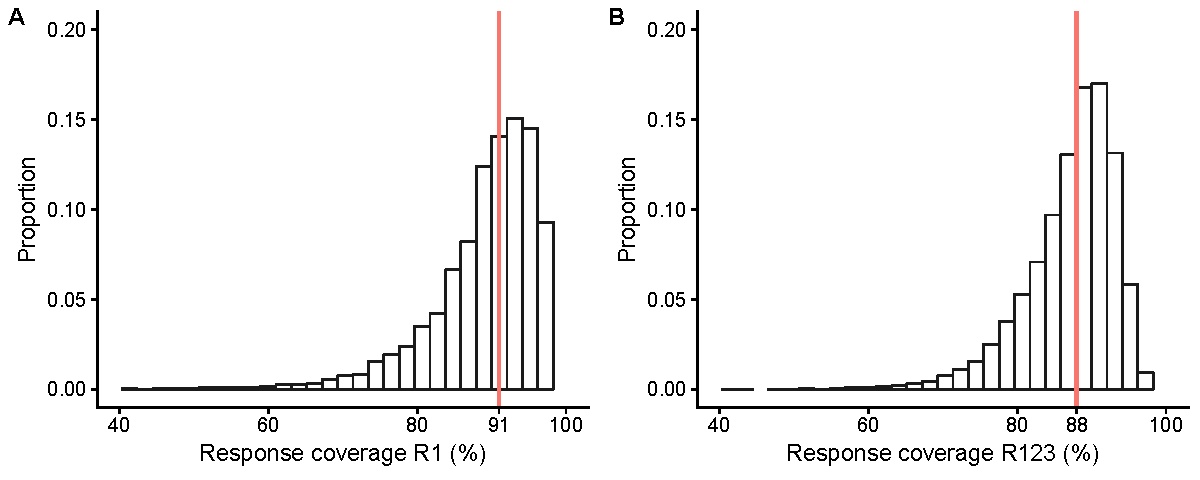
\includegraphics[width=14.5cm]{figures/responseCoverage.pdf}
  \caption{Density plot of the coverage based on single (R1) and continued responses (R123), where coverage in this context refers to the proportion of responses (to a specific cue) that belonged to the set of cue words in the strongly connected component. The proportion of responses retained for each cue is indicated by the \textit{x}-axis and shows that most cues retain about 90\% of their responses. }
  \label{figure:Coverage}
\end{figure}

How much data was lost by adopting this network representation? That is, given that we reduced the raw data R1 and R123 to graphs $G_{R1}$ and $G_{R123}$ that are defined over a set of 12,176 and 12,216 words respectively, it is natural to ask what proportion of participant responses are ``covered'' by this reduced representation. To calculate the coverage, we computed the average number of response tokens for each cue when only responses that are part of the strongly connected component are considered. Overall coverage was high. The average coverage for $G_{R1}$ was 0.89 with a median of 0.91 and the total distribution is shown in Figure~\ref{figure:Coverage}.
The proportion of word associations retained within the graph differed as a function of the cue word, ranging from 0.11 (\stim{pituitary}) to 1 (\stim{ache}). The average coverage for $G_{R123}$ equaled 0.87 with a median of 0.88, with values ranging from 0.41 (\stim{Homer}) to 0.99 (\stim{ache}). These numbers show that in both the single response and in the multiple response case the coverage is quite high: most responses that are generated by the participants were also part of the set of cues, and therefore were retained.



\subsection{Response chaining}
The use of a continued response paradigm makes it possible to investigate the possibility that people engage in response chaining --- using their own previous response as a cue or prime for their next response to the same word.\footnote{In this paper we do not discriminate between direct chaining (e.g., \stim{sibling} cues \stim{brother}, and \stim{brother} cues \stim{sister}), versus a ``latent variable'' account that views multiple responses as the outcome of a hidden concept (e.g., \stim{extremity} cues ``body extremity'' and ``body extremity'' cues both \stim{arm} and \stim{leg}). Although direct and hidden chaining may indeed represent different response processes, the data do not allow us to distinguish between them.} One effect of response chaining would be to increase the heterogeneity of the overall response distribution. In the (arguably unlikely) event that the later responses are completely unrelated to the original cue, this heterogeneity might be detrimental to the overall quality of the data. Alternatively, if the chained responses are still related to the original cue, the increased heterogeneity might be beneficial in eliciting additional knowledge possessed by participants, especially for cues that have a very dominant response. As an example, consider the cue word \stim{brewery} for which the response \stim{beer} occurs in 85\% of R1. In this case, it seems likely that \stim{beer} is dominating or blocking other strongly associated responses, and in such cases the continued procedure enables us to assess the full response distribution. In this section we investigate the extent to which response chaining is present, and what lexical factors at the level of the cue or the preceding response determine the amount of chaining.

\subsubsection{Evaluating chaining}
A simple way to test for response chaining is to compare the conditional probability of making a specific R2 response given that a particular R1 response was either made or not made. For instance, consider the example shown in Table~\ref{Table:contingency}. In this example the cue word was \stim{sun}, and we are interested in determining whether a participant is more likely to give \stim{star} as their second response if their first response was \stim{moon}. To do so, we exclude all cases where a participant gave \stim{star} as their first response, and then construct the 2x2 contingency table for R1 against R2 for all remaining participants. In this table the first responses are categorized as \stim{moon} or \stim{$\neg$moon} and the second responses are categorized as \stim{star} or \stim{$\neg$star}. If the first response does not act as a prime for the second response, there should be no association in this table. To test this we adopted a Bayesian approach for the analysis of contingency tables \citep{Gunel1974,Jamil2017}, assuming a joint multinomial sampling model. For the \stim{sun -- moon -- star} example, the resulting Bayes factor was $6.53\times 10^6$ in favor of an association, with an odds ratio of -3.88 (95\% CI: -5.97 to -2.45). In other words, in this example, we find very strong evidence for a chaining effect.


\begin{table}[t]
\centering
\caption{Contingency table for the cue \stim{sun} and the mediating effect of R1 = \stim{moon} on R2 = \stim{star}.
Note the sampling without replacement correction in the cell indicated with (*) obtained by removing the occurrences of star as R1. }
\label{Table:contingency}
\begin{tabular}{@{}rrrr@{}}
\toprule
& \multicolumn{2}{c}{R2} \\
\cmidrule(r){2-3}
R1 					& star 			& $\neg$ star 			& Total \\
\midrule
moon 				& 13 			& 12					& 25    \\
$\neg$ moon 		& 1 			& 74*					& 75 	\\
Total 			    & 14 			& 86					& 100   \\
\bottomrule
\end{tabular}
\end{table}

More generally, we calculated the corresponding Bayes factor (BF) for all possible \stim{cue -- R1 -- R2} triples. In approximately 1\% of cases we found strong evidence (Bayes factor $>$ 10) for response chaining. Examples of such \stim{cue -- R1 -- R2} triples are presented in Table~\ref{Table:chainingExamples}.  Moderate evidence (3 $<$ BF $<$ 10) was found for 19\% of cases. Some care is required when interpreting the ``moderate evidence'' cases, as the Bayes factor analysis yields moderate evidence anytime the R2 being tested never appeared as an R1, and as a consequence many of these weaker results may simply reflect the  increased heterogeneity in R2. While a more sophisticated approach could be adopted that incorporates R3, for the sake of brevity we simply note the possibility that a modest amount of response chaining exists in the data.

\begin{table}[t]
  \centering
  \caption{Top 10 mediated R2 responses for a specific cue and preceding response R1 together
  			with their Bayes factor and probability compared to no chaining.}
  \label{Table:chainingExamples}
  \begin{tabular}{rrrrr}
  \toprule
  	Cue & R1 & R2 & $log(BF_{10})$ & Probability \\
  \midrule
    gender    			& male     		& female   		& 16.31    	& 1.00 \\
    siblings    		& brothers 		& sisters   	& 14.29    	& 1.00 \\
    sibling 			& sister 		& brother 		& 13.65 	& 1.00 \\
    hop          		& skip 			& jump 			& 12.98 	& 1.00 \\
    parents 			& mother 		& father 		& 12.77 	& 1.00 \\
	extremity   		& arm 			& leg   		& 12.53    	& 1.00 \\
	condiments 			& salt 			& pepper 		& 11.80 	& 1.00 \\
	Korea 				& North 		& South 		& 11.73 	& 1.00 \\
	commence	 		& begin 		& start 		& 11.68 	& 1.00 \\
    sex					& male 			& female 		& 11.64 	& 1.00 \\

\bottomrule
  \end{tabular}
\end{table}

\section{Using association frequency to predict lexical processing}

The first half of this paper described a number of properties of the SWOW-EN dataset itself. In order to check the validity of the data, in the next part we examine how well the SWOW-EN data function as a predictor of other empirical data relative to other corpora. For example, it is typically assumed that response frequency (i.e., the number of times word $j$ is given as a response to cue word $i$) is related to the {\it strength} of the association between words $i$ and $j$, and as such should correlate reasonably well with other measures of semantic relatedness. Moreover, if we aggregate over all cues within the SWOW-EN, and simply consider the frequency with which word $j$ appears as a response, we should expect this to serve as a measure of the lexical centrality. That is, the frequency of a response provides us with an idea about which words are central or salient in the lexicon and might determine how efficiently lexical information can be retrieved.

To verify this, we used the response frequencies in the SWOW-EN data to predict three relevant behavioral measures. The first two measures were taken from the E-lexicon project \cite[http://elexicon.wustl.edu/]{BalotaYap2007}. They consisted of lexical decision and naming latencies for over 40,000 English words. The last measure was taken from the Calgary Semantic Decision (CSD) project \citep{PexmanHeard2017}, in which participants performed a binary concrete / abstract judgment for 10,000 English words.

We computed correlations to the SWOW-EN response frequencies using both the R1 data and the R123 data. For comparison purposes, we computed the same correlations for two additional word association norms (the USF norms and the EAT norms).
Because the number of responses per cue varied in the USF data (mean = 144, range = [39,203]), we sampled 100 responses per cue and removed 90 cues that had fewer than 100 responses. This reduced the total set of cues from 5018 to 4928.

Moreover, as word frequencies are one of the most powerful predictors of word processing speed \citep{BrysbaertNew2009} in a variety of tasks like lexical decision and naming, we also computed the correlation for the SUBTLEX-US norms, as these norms captured more variance than previously used word frequency norms available \citep{BrysbaertNew2009}.\footnote{The frequency norms were based on word forms, since \citet{BrysbaertNew2009} also reported that the advantage in terms of variance accounted for lemmas was minimal.}


\subsection{Analysis and results}

In keeping with previous studies \citep{BalotaYap2007,BrysbaertNew2009}, we used the $z$-transformed response times for the lexical decision data and the naming latency data. Additionally, in order to reduce skewness we log-transformed both the dependent and independent variables in our analyses. To do so, the $z$-scores were transformed to positive quantities by adding the minimum of the obtained $z$-scores; for centrality scores, a constant of 1 was added.

\begin{figure}[ht]
\centering
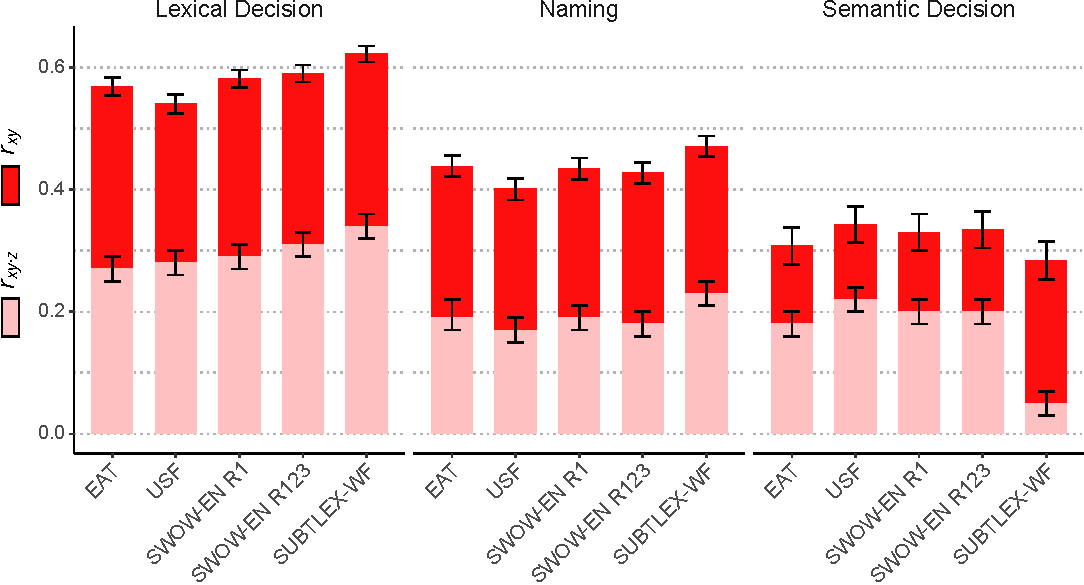
\includegraphics[width=14cm]{figures/LexicalProcessing.pdf}
\caption{Pearson correlations $r_{xy}$ and 95\% confidence intervals for naming and LDT data from the E-lexicon project and semantic decision latencies from the Calgary Semantic Decision (CSD) project (correlations multiplied by -1 for readability). Three different word-association datasets (EAT, USF and SWOW-EN) and one language-based measure of frequency derived from SUBTLEX are included. For the word-association datasets the partial correlations, indicated as $r_{xy\cdot z}$, are calculated given word frequency based on $z$ = SUBTLEX-WF; for SUBTLEX-WF, the partial correlation $r_{xy\cdot z}$ removes the effect of the word-association datasets.} \label{figure:frequencyCorrelation}
\end{figure}



The results of the correlation analyses are depicted graphically in Figure~\ref{figure:frequencyCorrelation} (red bars). The correlation of the lexical decision time and naming tasks is slightly higher for word frequencies (SUBTLEX-WF) than for any of the four word association datasets. This is not surprising insofar as the activation of semantic information in these tasks is limited. In contrast, for the semantic categorization task correlations were of similar size.

Given the broadly similar performance of word-association response frequency and word frequency as predictors in these tasks, a natural question to ask is whether the word association data encode any additional information not captured by word frequency. To that end we also calculated partial correlations between the association measures, after controlling for the word-frequency information in SUBTLEX-WF (and vice versa). The results are shown in pink in Figure~\ref{figure:frequencyCorrelation}, and show a similar pattern as before, with only modest differences between the four word-association norms. More importantly, they all show that a significant portion of the variance is not captured by word frequency. Curiously, the inverse relation does not necessarily hold, as can be seen in the far right of Figure~\ref{figure:frequencyCorrelation}: while word frequency does contain unique information for the lexical decision and naming tasks, it is almost entirely unrelated to semantic categorization after controlling for word association.

Taken together, these results suggest that the response frequencies in a word-association task do provide a valid index of lexical processing, and one that contributes considerable information over and above word frequency. In addition, we find that their usefulness depends on the nature of the task: word-association norms may be better suited as predictors (relative to word frequencies) for semantic tasks than for purely lexical tasks. Moreover, the fact that the results for SWOW-EN were at least as good as older norms is reassuring. It suggests that our continued-response procedure, combined with the larger cue set, did not strongly affect the validity of the association response counts, and that our more heterogeneous participant sample did not strongly affect the nature of the response frequencies.

\section{Using word associations to estimate semantic similarity}

In the previous section we sought to validate the SWOW-EN norms in a somewhat simplistic fashion, focusing on the overall response frequency for each word, aggregated across cues. It is reassuring that the aggregated data behave sensibly, but our expectation is that many interesting applications of SWOW-EN norms would rely on the specific \textit{patterns} of cue-response association. To illustrate how the SWOW-EN norms can be used in this fashion, we now consider word associations as measures of semantic similarity.\footnote{In the literature, ``similarity'' is often used as a more narrow term than ``relatedness''. In this article, we use the term relatedness to identify an existing association (i.e., a direct path) between a cue and target and use the term similarity to indicate the overlap in either direct or indirect neighbors they have (see further).} The focus on similarity reflects the importance that it plays within the psychological literature. Similarity is a central concept in many cognitive theories of memory and language. In priming, similarity between cue and target predicts the latency to process the target and the size of the priming effect depends on how similar the prime is\footnote{A systematic study of priming would bring together both the notion of association (forward and backward), spreading activation and distributional overlap. A full evaluation of semantic priming is beyond the scope of this article as it depends on many properties such as the inter stimulus interval or the nature of the task (naming or lexical decision. However,a preliminary analysis using data from the Semantic Priming Project \citep{HutchisonBalota2013} suggests that the findings for priming match those of lexical centrality and similarity where the performance of the new continued norms is as good or better than previously used norms.}. In various memory-related tasks like free recall, word associations are strong predictors of intrusion and recall performance \citep{Deese1959}. Representational similarity as measured by voxel analysis is also becoming increasingly important in neuro-imaging approaches that try to uncover the structure of semantic memory. Across a range of studies, the fMRI evidence indicates that the pattern of activation across different areas of the brain when reading common words \citep{Mitchell2008} can be predicted from distributional lexico-semantic models \citep{Schloss2016}. Against this backdrop, it seems sensible to consider how the SWOW-EN norms might be used to measure semantic similarity.


\subsection{Three measures of semantic similarity}

This section outlines three ways to estimate semantic similarity between a pair of words. These three measures vary systematically in terms of the amount of information they use -- in the simplest case we consider only the direct neighbors between two words, whereas in the most sophisticated case we consider the overall structure of the semantic network. We chose these three measures to highlight a tension in how word associations are used. For instance, the direct associative strength (i.e., association frequency) is often treated as a nuisance variable -- in the case of priming, tests of semantic facilitation are often addressed by \textit{controlling} for associative strength, while manipulating the semantic relatedness between two words \cite[see][for an extensive overview]{Hutchison2003}. In our view this is an unnecessarily limited approach, especially now that large datasets such as the SWOW-EN norms are available: as an alternative perspective, we suggest the association data themselves provide a strong indication of the similarity (and thus the meaning) of a word. Indeed, this point was highlighted in the seminal work of \citet[][p vii]{Deese1965}, who argued that
\begin{quote}
``The interest of psychologists in associations has always been misguided because the whole classical analysis of associations centered around the circumscribed and uninteresting problem of stimulus - response, of what follows what.''
\end{quote}
By focusing solely on the direct stimulus-response relationship between a pair of words, we end up ignoring the rich pattern of relationships that span the entire lexicon. It is this idea that we explore with the aid of our three measures of similarity.
Each of these measures reflects the number of paths shared between a cue and a target. The most common case is that where only the neighbors shared by cues and targets are considered. In this scenario, two words have a similar meaning if they share many neighboring nodes and we will use cosine similarity.

However, it is quite straightforward to extend the notion of relatedness to incorporate indirect paths connecting cues and targets as well, to capture a more global measure of relatedness. In the following section we will address both scenarios.



\subsubsection{Associative strength}

The simplest possible measure of semantic relatedness is to use the associative strength measure, $p(r|c)$, the probability of responding with word $r$ when given word $c$ as a cue. In this case, the relatedness is expressed as a weighted edge between cue and target. Since for most pairs of words such a path does not exist, the use of this measure is limited. Instead, we focus on ``local'' similarity based on the neighboring nodes they share. Given two cues, $a$ and $b$, and a total of $N$ different nodes, we measure their similarity $S$ as the cosine between them:

\begin{equation}
S(c_a,c_b) = \frac{\sum_{i=1}^N p(r_i|c_a) p(r_i|c_b)}
{\sqrt{\sum_{i=1}^N p(r_i|c_a)^2}\sqrt{\sum_{i=1}^N p(r_i|c_b)^2}}
\end{equation}

This cosine similarity measure reflects the shared neighbors between $a$ and $b$ and consists of a dot product of the associative response strengths in the numerator and divided by the L2-norm in the denominator. In contrast to other distance metrics such as Euclidean distances the denominator normalizes the magnitude of each vector, which makes both words comparable even when the amount of information for them differs.

We include local similarity based on strength primarily as a baseline measure of performance against judged similarity data when comparing it to global similarity measures derived from random walks which we will introduce in the next section

\subsubsection{Pointwise mutual information}

It has long been recognized that the simple frequency of response $p(r|c)$ is not an ideal measure of semantic similarity \cite[see p 10,][]{Deese1965}.  In recent years, an information theoretic measure based on the full distribution of responses to cue word $c$ -- the {\it positive pointwise mutual information} (PPMI) -- has been shown to predict the behavior in various language processing tasks \cite[e.g.,][]{Recchia2009}. We calculated the PPMI measure as follows:


\begin{equation}
\begin{array}{lcl}

\mbox{PPMI}(r|c)& = & \max\left(0, \log_2 \left(\frac{p(r|c)}{ p(r)} \right)\right) \\[10pt]
\mbox{PPMI}(r|c) & = & \max\left(0, \log_2 \left(\frac{p(r|c)}{ \sum_i p(r|c) p(c)} \right)\right) \\[10pt]
\mbox{PPMI}(r|c) & = & \max\left(0, \log_2 \left(\frac{p(r|c)N}{ \sum_i p(r|c)} \right)\right) \\[10pt]
\end{array}
\end{equation}

In the second line of the equation, the denominator takes into account how often a response is given for all cues $i$. In the last line of the equation we observe that the $p(c)$ is identical for all $c$ and equals $1/N$ where $N$ corresponds to the number of cues (or vertices) in the graph.
This way, responses that are given very frequently for many cues are considered less informative than responses that are given for only a small number of cues. In contrast to associative strength, this mutual information measure thus considers distributional information derived from the entire graph. In line with our previous work \citep{DeDeyne2016JEP,DeDeyne2016ACL}, we apply point-wise mutual information to the forward associate strengths. In light of the typical results in text-corpus based studies, we expect this approach to positively affect the performance in semantic tasks \citep{Bullinaria2007}. After weighting the responses according to Equation 2, we again calculated local similarity as the cosine overlap between two words.




\subsubsection{A random walk measure}
The PPMI measure of relatedness extends the simple associative strength measure by taking into account the full distribution of responses to a particular cue word, but it is still a ``local'' measure of similarity in the sense that it only considers the responses to that specific cue.
Taking a more ``global'' network perspective it is easy to see that similarity reflects more than just the immediate neighbors of a word, and could equally consider indirect paths or neighbors of neighbors as well, consistent with a spreading activation mechanism \citep{Collins1975}. In contrast to local similarity, a global similarity measure also considers the similarity among the neighbors themselves, leading to a recursive interpretation based on the idea that a node activates not only its neighboring nodes, but also the neighbors of these neighbors, though one would expect that these indirect relations contribute less to the overall similarity than the more salient direct relationships.

A formal implementation of this principle relies on a decaying random walk process \cite[see][]{AbbottAusterweil2015,BorgeHolthoeferArenas2010,DeDeyne2012Weak,Griffiths2007b} and is closely related to measures referred to as the Katz index, recurrence and the Neumann kernel \citep{Fouss2016} in other domains than psychology. In this paper we adopt the approach described in \citet{DeDeyne2016JEP}, and assume that the similarity between pairs of words is captured by the distributional overlap of the direct and indirect paths they share \citep{BorgeHolthoeferArenas2010,Deese1965,DeDeyne2014CorpusSize}.
For each node, this distributional representation constitutes a weighted sum of paths. More formally, consider a walk of a maximum length $r = 3$, where $\mathbf{I}$ is the identity matrix and the damping parameter $\alpha < 1$ governs the extent to which similarity scores are dominated by short paths or by longer paths \citep{Newman2010}:

\begin{equation}
\begin{array}{lcl}
\mathbf{G_{rw}}^{(r=1)} & = & \mathbf{I},\\
\mathbf{G_{rw}}^{(r=2)} & = & \alpha \mathbf{P} + \mathbf{I},\\
\mathbf{G_{rw}}^{(r=3)} & = & \alpha^2\mathbf{P}^2 + \alpha\mathbf{P} + \mathbf{I}\\
\end{array}
 \label{equation_iteration}
\end{equation}

\noindent
During each iteration, indirect links reflecting paths of length $r$ are added to the graphs. Longer paths receive lower weights because of the exponent $r$ of $\alpha$. In the limit, we arrive at a simple representation based on the inverse of the transition matrix:

\begin{equation}
\begin{array}{lcl}
\mathbf{G_{rw}}  = \sum_{r =0}^{\infty}(\alpha\mathbf{P})^r  =   (\mathbf{I} - \alpha \mathbf{P})^{-1}
\end{array}
\label{equation_RW_algebraic}
\end{equation}
\noindent

A common problem is that such a walk will also be biased toward nodes that are highly connected \citep{Newman2010}. To address this, the matrix $\mathbf{P}$ is constructed by applying the PPMI transformation to the raw association data and normalizing the values to sum to 1. Finally, like the local measure of similarity, we then take the cosine of the PPMI row-normalized $G_{rw}$ distributions to calculate the similarity of two words.

\subsection{Benchmark data}

To evaluate these measures of similarity, we rely on seven existing datasets in which participants judged the similarity of word pairs. We briefly describe these data \citep[see also][]{DeDeyne2016ACL}. In one study, SimLex-999 \citep{Hill2016simlex}, subjects were explicitly asked to judge the {\it similarity} between words ignoring their potential relatedness. In the remaining studies participants were asked to judge the relatedness of word pairs using rating scales. These include the WordSim-353 relatedness dataset \citep{AgirreAlfonseca2009}, the MEN data \citep{BruniBoleda2012}, the Radinsky2011 data \citep{RadinskyAgichtein2011}, the popular RG1965 dataset \citep{Rubenstein1965}, the MTURK-771 data \citep{HalawiDror2012} and Silberer2014, a large dataset consisting of mostly concrete words \citep{Silberer2014}.

Because the SWOW-EN dataset contains capitalization, proper capitalization was restored in a number of evaluation sets. Similarly, we checked the occurrence of proper nouns among the EAT and USF cues and applied capitalization where appropriate. We also checked the spelling mistakes and variants and corrected mistakes or converted to American English to ensure maximal overlap between the datasets.


\subsection{Results and discussion}
The performance of all three similarity measures is shown for each of the seven studies Figure~\ref{figure:SWOWSimilarity} and in Table~\ref{Table:simDetailed_SWOW}, which tells a very consistent story. Regardless of whether the measures are computed using R1 data or R123 data, the PPMI measure always outperforms the simpler associative strength measure, and the random walk model always performs at least as well as the PPMI measure, but usually performs better.

\begin{figure}[!ht]
\centering
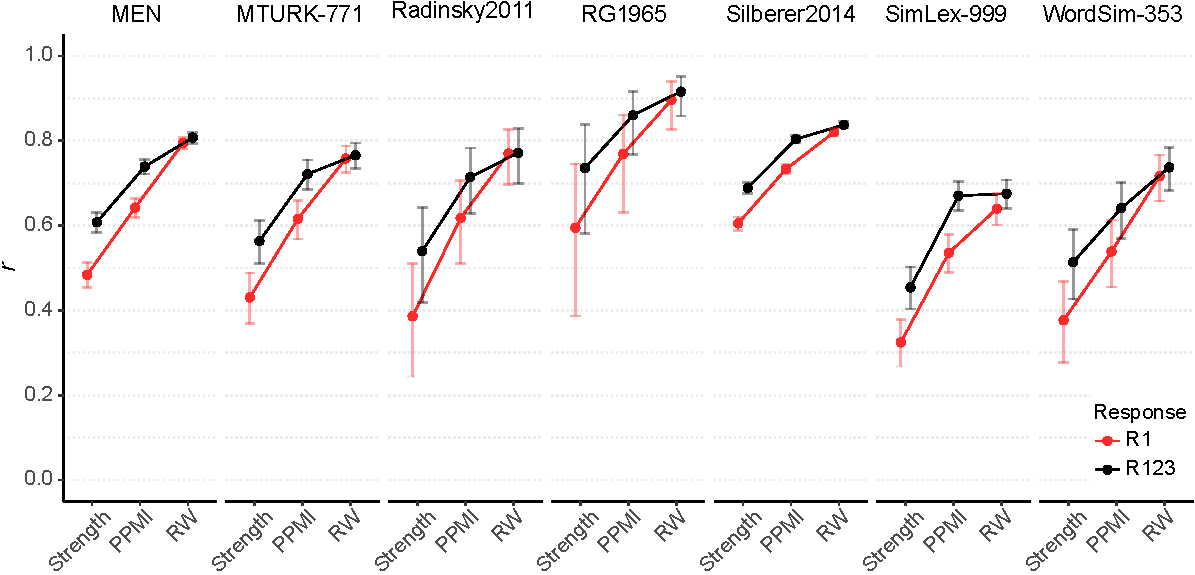
\includegraphics[width=14.8cm]{figures/SimilarityComparison.pdf}
\caption{Pearson correlations and confidence intervals for judged similarity and relatedness across seven different benchmark tasks. Predictions are based on either local similarity using associative strength, PPMI, or global similarity-based random walks (RW). Graphs including the first responses ($G_{R1}$) and all responses ($G_{R123}$) show how similarity interacts with the density of the graph.} \label{figure:SWOWSimilarity}
\end{figure}


For the associative strength and (to a lesser extent) PPMI measures, the larger dataset based on R123 leads to better predictions than the first response only data in R1, though this effect is almost completely attenuated for the random walk measure. There are some differences among the various datasets --- most measures performed worst on the SimLex-999 dataset, in which participants were explicitly trained to ignore relatedness when judging word pairs --- but even in this case the same pattern of performance is observed.

Extending this analysis, we repeated the procedure above for the USF norms, the EAT norms, and an aggregated dataset that pooled the USF norms with the SWOW-EN norms. The results are shown in Figure~\ref{figure:SWOWUSFEAT} and Table~\ref{Table:simSummary_SWOW}.
For reasons of conciseness, this table only presents the (micro-)averaged correlation across all seven datasets. The pattern of results is similar, despite that only half of the similarity pairs were present in all three word association datasets. In general, measures of similarity-based on EAT, USF and the R1 data from SWOW-EN perform similarly, while the larger R123 data from SWOW-EN yields somewhat better performance. Finally, there is no evidence that combining the USF and SWOW-EN R123 norms together improves performance, as the red curves in Figure~\ref{figure:SWOWSimilarity} illustrate.

\begin{figure}[!ht]
\centering
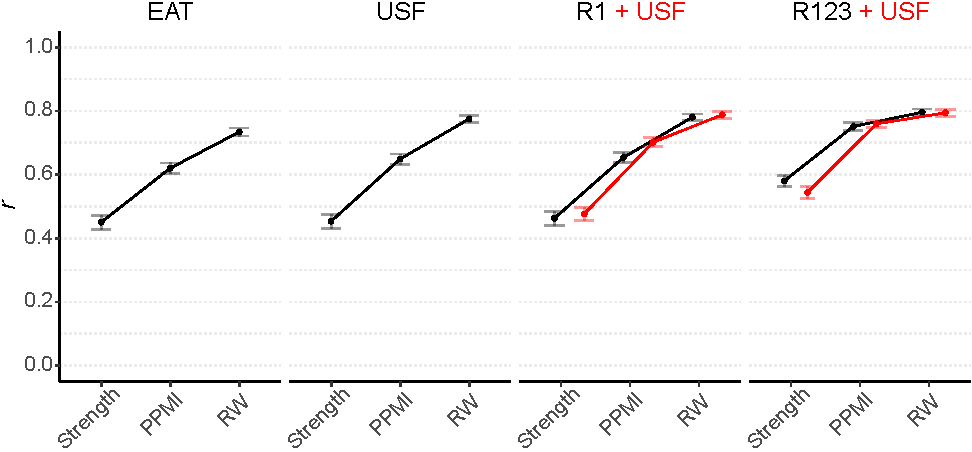
\includegraphics[width=12cm]{figures/SimilarityDatasets.pdf}
\caption{Comparison between two existing datasets (EAT and USF) and SWOW-EN in predicting human similarity and relatedness judgments. Pearson correlations and confidence intervals reflect micro-averaged judgments across seven benchmark tasks. Predictions are based on either local similarity using associative strength, PPMI, or global similarity based random walks (RW). In addition to the three association datasets, a combination of USF and SWOW-EN (red curves) is included as well showing that adding more data does not markedly improve the results.} \label{figure:SWOWUSFEAT}
\end{figure}

Overall, the results strongly favor the random walk approach, especially when sparsity of the data is an issue. The findings are in line with our previous work examining how people make judgments about very weakly related words \citep{DeDeyne2016JEP} and with other recent approaches that show how indirect paths contribute to semantic similarity \citep{KenettEffi2017}. Returning to Deese's (1965) comments quoted earlier, the central intuition --- namely that the simple stimulus-response contingencies are the {\it least} interesting aspect to word association data --- seems to be borne out.


\section{General Discussion}

In this article, we have presented a new dataset for English word associations. It was constructed to capture a large portion of the mental lexicon by including over 12,000 cue words and 300 associations for each of these cues. It includes the cues of the USF dataset, which will facilitate further replications of previously obtained results, but doubles the number of available responses per cue. Because the total number of cues is considerably larger than previous datasets, it is possible to derive an accurate semantic network based on cue words only. The biggest advantage of this is that it opens up a variety of new analyses that take into account the overall structure of the cue-based  semantic network, some of which we have briefly outlined in this paper.


\subsection{The importance of rich association networks}

One of the main points we have emphasized throughout is the importance of considering association in context. This was especially evident when using word associations to predict semantic relatedness. As we have seen, the predictive power of the norms varies considerably depending on the density of the word association networks used, and the amount and weighting of the information encoded in the entire network. There is an enormous difference between the worst performing measure and the best. When a random walk measure is based on the SWOW-EN R123 data, we obtain good predictions about semantic relatedness ($r=.81$). Moreover, it is possible to produce good predictions when a more sophisticated model (random walk) is applied to comparatively impoverished data such as the EAT ($r=.73$), and similarly, it is possible to get by with simplistic measures (associative strength) when given rich data like SWOW-EN R123 ($r=.64$). However, when the data are less rich (EAT) and the measure is based on distributional overlap based on simple associative strength, the predictive power declines drastically, and the overall correlation with semantic relatedness is a mere $r = .46$.

The ability to produce quantitatively better predictions matters in a number of areas.
Many categorization accounts predict prototypicality by considering how similar category exemplars are to each other. Word associations offer a way to estimate such prototypicality \citep{DeDeyne2008}. Likewise, estimates of similarity are also the key component in predicting other aspects of word meaning such as connotation based on valence, arousal and potency, concreteness or even age-of-acquisition. In these cases as well, our findings suggest that word associations often out-perform predictions based on the most recent text models \citep{DeDeyne2016ACL,VanRensbergen2016,Vankrunkelsven2018} using a very sparse representation.
More generally, we expect that these findings will be useful across a range of studies about psychological meaning, including priming studies and patient studies where semantic effects might be small and go undetected when the relatedness reflects distributional properties in external language.



\subsection{Comparison to other measures and approaches}

It is unlikely that word association measures will always provide the best tool for studying semantic representation, and some comments about the relationship to other approaches are worth making. For instance, we found that association response frequency correlates only moderately with word frequency ($r = .54$), and while word association data seem well suited to semantic categorization and semantic relatedness, word frequency measures (based on the SUBTLEX-US data) performed better as predictors of lexical decision times and naming (but see further). That being said, in contrast to other subjective techniques to elicit meaning, the information captured by an unconstrained  word association task does seem to capture the {\it right kind} of meaning; meaning that is not limited by defining, characteristic, or entity features, but meaning that reflects mental representations that include properties about connotation, scripts and themes, properties notably absent from other subjective measures such as feature norms \citep{DeDeyne2008,McRae2005}.

To verify if this indeed the case, we performed an additional analysis comparing similarity benchmark data introduced earlier and two publicly available feature sets: the McRae feature norms for 541 nouns \citep{McRae2005} and the CSLB feature norms for 637 words \citep{Devereux2014}. For conciseness, we only compared them to the similarity estimates of SWOW-EN using all responses with spreading activation strengths. Since most of these norms are collected for concrete norms, only two studies, Silberer2014 and MEN, had sufficient overlap with the stimuli in the feature norms. Similarity was calculated in a standard way, using the cosine overlap of the feature vector, where each entry corresponds to the number of participants that gave the feature for the concept.
Using the McRae norms the results were  $r(65) = .64, CI = [.47,.77]$ for MEN and $r(2392) = .77, CI = [.75,.79]$ for Silberer2014. For SWOW-EN the results were $r(65) = .85, CI = [.76,.90]$ and $r(2392) = .85, CI = [.84,.86]$ for the same datasets.  For the CSLB norms we found $r(132) = .70, CI = [.60,.78]$ for MEN and $r(3126) = .80, CI = [.79,.81]$ for Silberer2014. Again, the correlations were higher for SWOW-EN, $r(132) = .90, CI = [.86,.93]$ and $r(3126) = .86, CI = [.85,.86]$ for MEN and Silberer2014 respectively. In short, these findings suggest that concept feature norms only partly capture meaning involved similarity judgments as well. More generally, it suggests that word-association norms provide a more reliable alternative for concept feature norms for a wide variety of words and potentially the best semantic measure available to date.

Looking beyond measures based on experimental tasks, there are many lexico-semantic models that rely on naturalistic text corpora as their input data, typically using some form of dimensionality reduction to extract a semantic representation \citep[see][for an overview]{Jones2015}. Here as well, word associations outperform text-based semantic models. Previous work using largely the same benchmarks presented here showed that the best-performing text-model resulted in a correlation of $r = .69$, which was significantly lower than that of the best-performing word association model, $r = .82$ \citep{DeDeyne2016ACL}.

Apart from their ability to predict, it is also important to consider \textit{what kind} of theoretical contribution subjective measures of meaning can make, especially as improved objective measures of language from corpora are becoming available.
Some researchers have argued that word association measures correspond to \textit{empty} variables \citep[as discussed in ][]{Hutchison2008}. The underlying idea is that the processes involved in generating them are likely to match other processes in commonly used tasks such as priming or similarity ratings. If so, this might explain their good performance in comparison to objective text-based measures \citep[e.g.,][]{JonesHills2015}. At the same time, researchers have criticized word associations to be underpowered as well, because they only capture the most dominant responses, whereas the amount of text that can be encoded in text-based models is virtually limitless which allows for the explicit encoding of weak co-occurrence relations \citep{Roelke2018}.

Our findings speak to both of these conjectures. First of all, we agree that when causal claims about the nature of semantic cognition are the objective, the  question of circularity should be taken seriously. Even so, it is far for clear whether circularity through shared processes leads to better predictions. Assuming that some processes might be shared across different subjective tasks there are many reasons why prediction might be suboptimal. Specific biases (e.g., a frequency bias) might mask the content of representations, or the subjective judgments might be idiosyncratic  or fail to capture weak connections. Furthermore, a priori it is not clear whether the type of responses found in associations are appropriate, and perhaps more restrictive subjective tasks such as concept feature generation are more predictive when in comes to tasks tapping directly into word meaning.
What we find is that strength measures typically provide a poor account of relatedness or similarity,  and preliminary analyses on priming. However, measures that incorporate indirect informative relations systematically outperform simple strength-based measures. As noted earlier, this was clearly demonstrated when comparing the current norms with USF, where we found that spreading activation almost completely compensates the fact that only dominant responses are encoded explicitly.

Apart from the conclusions that can be drawn from inference using very little data, there might be a more important factor underlying the success obtained using word associations. A recent study found that the performance of word associations was mainly due to the fact that for concrete concepts word associations provide more grounded representations than do text models. The same study also evaluated emotional grounding in abstract words. There as well, a sizable advantage of associations relative to text-based representations can be explained because word associations accurately capture crucial emotive factors such as valence and arousal in abstract words, which make up the majority of the words in our lexicon \citep{DeDeyne2018VISEMO}.

Altogether, this suggests that studying word associations can reveal properties about both the processes and nature of the representations involved in semantic cognition.
While understanding the formation of word associations itself is an aspirational goal (and supported by the convergent validity provided in our findings), it would involve a perceptual (and emotional) grounded model, where modal specific representations are notoriously hard to obtain in an unsupervised or objective fashion. For example, the best-performing multimodal models are supervised learning models trained on human on naming data \citep[e.g.,][]{Bruni2014JAIR,Silberer2014}.  For now, even the most recent text-based lexico-semantic models provide only weak to moderate correlations with word associations. A representative example is a recent study by \citet{Nematzadeh2017} in which the highest correlation obtained across a variety of text-based models (including topic and word embedding models) were used to product word associations was .27.

As text-based approaches of semantic cognition continue to improve, it is also becoming increasingly clear that more stringent criteria to evaluate them are needed.
One of the challenges is that much larger amounts of text might be over-fitting the behavioral data  leading to erroneous conclusions about what kind of representations language contributes to. An example is the capacity of extremely large text models to encode some modal-specific representation \citep{Louwerse2011TiCS}. Apart from the issue whether their size is appropriate, this example also illustrates the difficulty of proving the unique (causal) contribution given the overlap with abundantly available modal-specific perceptual information that is also contributing to our mental representations through processes of perceptual simulation or imagery. In areas such as these, both subjective internal and objective external measures can contribute to our understanding of word processing and semantic cognition and taking a dialectic approach of comparing internal and external language representations might provide a way forward towards understanding the nature of our mental representations.


\subsection{On differences between norms}

Throughout the paper we have observed small but consistent differences between the older USF and EAT norms and the newer SWOW-EN dataset. In many cases, the differences are simply a matter of scale: the SWOW-EN dataset is much larger than earlier norms, and in some cases this may provide an advantage. However, it is worth noting some of the other differences between the dataset. The current sample is without doubt more heterogeneous than the EAT and USF samples, which were collected predominantly among college students.

It is very likely that performance will be higher in studies in which there is a close match in participant demographics with any given word association dataset. For example, we expect that the associations in USF will provide a good match when the participants are American college students. Besides demographic differences and the obvious difference between our continued response task and the more traditional single response task there are other differences that need to be pointed out as well.

One notable difference lies in the task instructions. The instructions we used were designed to elicit free associations in the broadest possible sense, whereas in the USF norms \citet{Nelson2004} participants were asked to write down the first word that came to mind that was ``meaningfully related or strongly associated to the presented cue word.'' The fact that participants were asked to give a {\it meaningful} response might affect the type of responses that are generated. There is some indication that this indeed might have resulted in a different type of response, for example by considering the number of times participants make reference to proper nouns (names of people, movies, books, etc), which are not that common in the USF norms. The selection of cue words itself is likely to have contributed to this as well, as the current set also included a small number of proper nouns, which might have indicated to the participant that such words were also valid responses. When we consider the EAT, the differences in methodology and sample are somewhat more pronounced. Not only are the EAT data older, they were collected from British speakers that differed on other demographic measures also (students between 17 and 22, of which 64\% were male). The instructions for EAT asked participants to write down for each cue the first word it made him or her think of, working as quickly as possible \citep{Kiss1973}.

Perhaps it comes as a surprise that in light of all these differences, the three datasets often produce similar levels of performance. It is especially noteworthy that measures of semantic relatedness based on a ``spreading activation'' measure proved to be highly robust to differences in the datasets, again highlighting the value of using a method that incorporates information about the global structure of the semantic network.\footnote{To further illustrate this point, we correlated the predicted relatedness for the stimulus pairs of the seven studies described in the previous section and compared how similar these predictions were among models and found a correlation of .90 between the USF and the comparable SWOW-EN norms using the global random walk measure based on the first response, whereas the correlation was lower for the local similarity measures: .84 for associative strength weights, .78 for PPMI.}

A final point to make when comparing different norms --- one that we have not focused on in this paper --- is to consider the differences between the English language data (SWOW-EN) and the Dutch language data reported previously (SWOW-NL). The literature on word processing shows a strong English-language bias and some effects might be language specific. While we have previously investigated Dutch word associations and found similar results for relatedness \citep{DeDeyne2016JEP,DeDeyne2014CorpusSize}, centrality effects in lexical processing were better predicted by association response frequencies in Dutch, even though external word frequency norms were also based on SUBTLEX subtitles in Dutch \citep{DeDeyne2013}. There might be a number of factors underlying this observation, such as systematic language differences, demographic differences or even differences in the quality of the word frequency predictors. However, without further systematic research, any claims in this area remains largely speculative.


\subsection{Future work}
While we have focused our comparison mostly on previous English word associations, one of the goals of the current project is to collect these data for the most common languages in the world.
So far the largest resource is the Dutch SWOW-NL, which currently contains over 16,000 cue words and good progress is made on a similar Mandarin Chinese project, for which we collected at least 50 participants generated three associates to each cue, for over 8,500 cues.

In future research, we plan on extending the English database along two major lines. First, we have omitted the discussion of response latencies for word associations. Although these are now standard collected across the different SWOW projects, a full treatment of the use and properties of these latencies derived from the continued word association task would be beyond the scope of this article. Second, it would be good to keep extending the words included, especially as new words are introduced in the language. However, our results indicate diminishing returns for adding a large number of new cues that are likely low frequency. Instead, it might be useful to further elaborate on the different English variants (e.g., British and American) or supplement them with age-balanced data.
We also expect that better methods and models could further enhance the use of word associations. For example, in the current work a subject's primary, secondary and tertiary responses were simply added, which in some cases might introduce a bias. Other ways of calculating associative strength over multiple responses by non-linearly weighting responses and considering sampling without replacement for secondary and tertiary responses might be better suited \citep{DeDeyne2013c,Maki2008}. As demonstrated in the current work, some degree of response chaining will need to be considered as well.

Finally, in most research based on subjective or language corpora, we assume that the language or responses averaged over a large sample of speakers captures representations at the individual level as well. Evidence across a wide range of studies with different speakers suggests this is indeed the case.
While language and its communicative role might be special in providing a pressure to align our linguistic representations between different individuals, many interesting questions about individual differences remain unanswered. Partly, this has to do with the difficulty to collect large samples of language from an individual. However, recent work suggests that studying individual networks might be feasible \citep{Austerweil2012,Morais2013} and ongoing work to extend this approach is currently ongoing.
Altogether, we cannot help but agree with the closing paragraph by \citet[][p. 406]{Nelson2004} in the context of the USF norms: ``Difficult as they are to collect, such norms offer better maps for predicting performance in certain cognitive tasks, and if anything, more norms are needed.''

\newpage
\begin{appendix}
\section{Supplemental Tables}

\begin{table}
\begin{center}
\begin{small}
\caption{{\small Pearson correlation for seven judged relatedness and similarity studies, using three theoretical measures of similarity (strength, PPMI and random walk) constructed using either R1 or R123 responses from SWOW-EN. The ``micro-averages'' across datasets adjust for sample size by standardizing the ratings in each study and then correlating pooled data with theoretical predictions.}}
\label{Table:simDetailed_SWOW}
\begin{tabular}{@{}lrccclccccccc@{}}
\toprule
 & \multicolumn{1}{l}{} & \multicolumn{11}{c}{\textbf{SWOW-EN R1}} \\ \cmidrule(l){3-13}
 & \multicolumn{1}{l}{} & \multicolumn{3}{c}{Strength} &  & \multicolumn{3}{c}{PPMI} & \multicolumn{1}{l}{} & \multicolumn{3}{c}{RW} \\ \cmidrule(lr){3-5} \cmidrule(lr){7-9} \cmidrule(l){11-13}
Dataset & \textit{N} & \textit{r} & \multicolumn{2}{c}{\textit{CI}} & \multicolumn{1}{c}{\textit{}} & \textit{r} & \multicolumn{2}{c}{\textit{CI}} & \textit{} & \textit{r} & \multicolumn{2}{c}{\textit{CI}} \\ \cmidrule(lr){3-5} \cmidrule(lr){7-9} \cmidrule(l){11-13}
MEN	 			& 2706	 & .48	 & .45	 & .51	 & \multicolumn{1}{c}{} 	& .64	 & .62	 & .66	 & 	 & .79	 & .78	 & .81 \\
MTURK-771	 	& 716	 & .43	 & .37	 & .49	 & \multicolumn{1}{c}{}	 	& .62	 & .57	 & .66	 & 	 & .76	 & .73	 & .79 \\
Radinsky2011	& 158	 & .39	 & .24	 & .51	 & \multicolumn{1}{c}{} 	& .62	 & .51	 & .71	 & 	 & .77	 & .70	 & .83 \\
RG1965	 		& 53	 & .60	 & .38	 & .74	 & \multicolumn{1}{c}{} 	& .77	 & .62	 & .86	 & 	 & .90	 & .82	 & .94 \\
Silberer2014	& 6404	 & .61	 & .59	 & .62	 & \multicolumn{1}{c}{}	 	& .73	 & .72	 & .74	 & 	 & .82	 & .81	 & .83 \\
SimLex-999	 	& 988	 & .33	 & .27	 & .38	 & \multicolumn{1}{c}{}	 	& .54	 & .49	 & .58	 & 	 & .64	 & .60	 & .67 \\
WordSim-353		& 311	 & .38	 & .28	 & .47	 & \multicolumn{1}{c}{} 	& .54	 & .46	 & .61	 & 	 & .72	 & .66	 & .77 \\
\cmidrule(lr){3-5} \cmidrule(lr){7-9} \cmidrule(l){11-13}
Micro AVG       & 11336& .53 & .52 & .54 &  & .68 & .67 & .69 &  & .79 & .78 & .80 \\
 & \multicolumn{1}{l}{} & \multicolumn{11}{c}{\textbf{SWOW-EN R123}} \\ \cmidrule(l){3-13}
 & \multicolumn{1}{l}{} & \multicolumn{3}{c}{Strength} &  & \multicolumn{3}{c}{PPMI} & \multicolumn{1}{l}{} & \multicolumn{3}{c}{RW} \\ \cmidrule(lr){3-5} \cmidrule(lr){7-9} \cmidrule(l){11-13}
Dataset & \textit{N} & \textit{r} & \multicolumn{2}{c}{\textit{CI}} & \multicolumn{1}{c}{\textit{}} & \textit{r} & \multicolumn{2}{c}{\textit{CI}} & \textit{} & \textit{r} & \multicolumn{2}{c}{\textit{CI}} \\
\cmidrule(lr){3-5} \cmidrule(lr){7-9} \cmidrule(l){11-13}
MEN	 			& 2706	 & .61	 & .58	 & .63	 & \multicolumn{1}{c}{}	 & .74	 & .72	 & .76	 & 	 & .81	 & .79	 & .82 \\
MTURK-771	 	& 716	 & .56	 & .51	 & .61	 & \multicolumn{1}{c}{}	 & .72	 & .68	 & .75	 & 	 & .77	 & .73	 & .79 \\
Radinsky2011	& 158	 & .54	 & .42	 & .64	 & \multicolumn{1}{c}{}	 & .71	 & .63	 & .78	 & 	 & .77	 & .70	 & .83 \\
RG1965	 		& 53	 & .74	 & .58	 & .84	 & \multicolumn{1}{c}{}	 & .86	 & .76	 & .92	 & 	 & .92	 & .86	 & .95 \\
Silberer2014	& 6404	 & .69	 & .67	 & .70	 & \multicolumn{1}{c}{}	 & .80	 & .80	 & .81	 & 	 & .84	 & .83	 & .85 \\
SimLex-999	 	& 988	 & .45	 & .40	 & .50	 & \multicolumn{1}{c}{}	 & .67	 & .64	 & .70	 & 	 & .68	 & .64	 & .71 \\
WordSim-353	 	& 311	 & .51	 & .43	 & .59	 & \multicolumn{1}{c}{}	 & .64	 & .57	 & .70	 & 	 & .74	 & .68	 & .78 \\
\cmidrule(lr){3-5} \cmidrule(lr){7-9} \cmidrule(l){11-13}
Micro AVG       & 11336& .63 & .62& .64 &  & .77 & .76 & .77&  & .81 & .80 & .81\\
\bottomrule
\end{tabular}
\end{small}
\end{center}
\end{table}

% Checked
\begin{table}
\centering
\caption{Pearson correlation based on micro-averages over $N = 5,202$ items of seven datasets involving similarity judgments and relatedness derived from EAT, USF and SWOW-EN.
The columns refer to the role of weighting (associative strength or positive point-wise mutual information or PPMI) and spreading activation using random walks (RW).
The last two rows show the results for combined datasets through the intersection of cues found and single responses from USF and SWOW-EN.}
\label{Table:simSummary_SWOW}
\begin{tabular}{lccccccccccc}
\hline
$N$ = 5202 & \multicolumn{3}{c}{\textbf{Strength}} & \multicolumn{1}{l}{} & \multicolumn{3}{c}{PPMI} & \multicolumn{1}{l}{} & \multicolumn{3}{c}{\textbf{RW}} \\
\hline
Dataset & \textit{r} & \multicolumn{2}{c}{\textit{CI}} & & \textit{r} & \multicolumn{2}{c}{\textit{CI}} & & \textit{r} & \multicolumn{2}{c}{\textit{CI}} \\
\cline{2-4} \cline{6-8} \cline{10-12}
EAT	 				& .45	 & .43	 & .47	 & 	 & .62	 & .61	 & .64	 & 	 & .73	 & .72	 & .75 \\
USF	 				& .45	 & .43	 & .47	 & 	 & .65	 & .63	 & .66	 & 	 & .77	 & .76	 & .79 \\
SWOW-EN R1	 		& .46	 & .44	 & .48	 & 	 & .65	 & .64	 & .67	 & 	 & .78	 & .77	 & .79 \\
SWOW-EN R123	 	& .58	 & .56	 & .60	 & 	 & .75	 & .74	 & .76	 & 	 & .80	 & .79	 & .81 \\
\\
USF + SWOW-EN R1	& .48	 & .46	 & .50	 & 	 & .70	 & .69	 & .72	 & 	 & .79	 & .78	 & .80 \\
USF + SWOW-EN R123	& .54	 & .52	 & .56	 & 	 & .76	 & .75	 & .77	 & 	 & .79	 & .78	 & .80 \\
\hline
\end{tabular}
\end{table}

\FloatBarrier


\section{Terms of use and online materials}

\subsection{Fair use and referencing the data}
The data can be used for research purposes only. It is subject to a Creative Commons Attribution-NonCommercial-NoDerivs 3.0 Unported License and can not be redistributed or repackaged without explicit consent from the first author. When using these data please refer to them as the SWOW-EN2018 word association data and unless needed, use the corrected version for consistency. This project is a work in progress so if you find these data useful, please consider sharing our study:\\
\url{https://smallworldofwords.org/}


\subsection{Available resources}

\subsubsection{Original and processed data}
The main resources made available at \url{https://smallworldofwords.org/project/research/} consist of files with the original and processed data as used in this manuscript..
The original unprocessed data file contains both participant and response information. It consists of the complete raw uncorrected responses and cues. These data might be useful for those interested in spelling mistakes or would like to experiment with other ways of normalizing responses.
Each row in the file consists of participant and response data. The participant data include a unique participant identification number, age, gender, education, city and country details, native language and test date and time. The response data consist of the cue, the first response (R1), the second response (R2) and the third response (R3). For each of the three responses, the original and spell-checked responses are included.

The second file is derived from the raw data and consists of spell-checked cues and responses after removing participants that did not meet selection criteria. In contrast to the previous file, each cue has exactly 100 R1, R2 and R3 responses.  As described in the text, the responses were also Americanized. We propose to use these data as much as possible to facilitate comparison between results and refer to this dataset as the SWOW-EN2018 data.

In addition, we also provide a list with manually annotated spelling errors and welcome any suggestions to further extend this list. The scripts to process the data and calculate the measures reported in this paper can be obtained from \url{https://github.com/SimonDeDeyne/SWOWEN-2018}.

\end{appendix}
\bibliography{simon11}
\end{document}
